\documentclass[11pt]{article}
\usepackage[english]{babel}
\usepackage[utf8]{inputenc}
\usepackage[T1]{fontenc}
\usepackage{float}
\usepackage{lmodern,amsmath,amssymb,amstext,amsfonts,mathrsfs,graphicx,caption, subcaption}
\usepackage[width=14cm]{geometry}
\usepackage[colorlinks,pdfpagelabels,pdfstartview = FitV,bookmarksnumbered = true, bookmarksopenlevel=section, linkcolor = black,hypertexnames = false,citecolor = black,pdfpagelabels=false]{hyperref}
\usepackage{tablefootnote}
%\usepackage{rotating}
\usepackage{textcmds, enumitem}
\usepackage{sidecap} %, indentfirst
\usepackage[labelfont={bf,sf},font={small},labelsep=space]{caption}
\usepackage{chngcntr} % 			** Damit die Bilder Tabellen und Gleichungen 
\counterwithin{figure}{section}	%	** alle nach Kapiteln nummeriert sind.
\counterwithin{table}{section}%		**
\counterwithin{equation}{section}%	**	
\begin{document}
	
	\section{Methods}
	% Introduction.
	In this chapter, we will give an overview about the recurrent network (RNN) models for exploration of the feedforward recurrent alignment hypothesis that are evolved in this work. The firstly introduced symmetric network model builds the basis for modifications and extensions in other further models. The modified models will be introduced subsequently. Finally, we consider the role of learning could play in the feedforward recurrent alignment hypothesis. 
	
	\subsection{Symmetric Recurrent Network Model}
	% General Information about symmetric interaction network. 
	Due to the well understood mathematical characters of symmetric RNNs, they are often applied in models for neuroscience for a better understanding of certain dynamics.  
	Therefore, we firstly consider the basic case of having a symmetric recurrent network, which has the symmetric interaction matrix. For symmetric RNNs, if there is a connection between two neurons $n_i$ and $n_j$, the strength of the directed connection from the neuron $n_i$ to the neuron $n_j$ equals the directed connection from $n_j$ to $n_i$. 
	% A figure for network construction.
		\begin{figure}[H] \label{fig:symmetric_RNN}
			%\centering
			\begin{subfigure}[b]{0.4\textwidth}
				\centering
				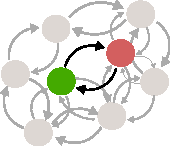
\includegraphics[width=0.2\textheight]{../figures/sym_net.pdf}
				\vspace{0.2cm}
				%\caption{Example of symmetric connections between two neurons.}
				\caption{}
			\end{subfigure}
			\hspace{0.4cm}
			\begin{subfigure}[b]{0.4\textwidth}
				\centering
				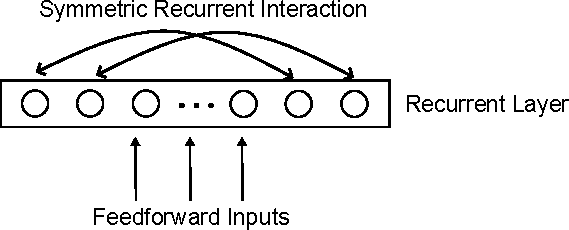
\includegraphics[width=0.4\textheight]{../figures/recurrent.pdf}
				%\caption{Structure of a recurrent network (RNN)}
				\caption{}
			\end{subfigure}
		\caption{\textbf{Illustration of symmetric recurrent networks (symmetric RNNs).} \\ \textbf{(a)} An example of symmetric connections between two neurons in a network with multiple neurons. If there are connections between two neurons, here for example the green and red neurons, the directed connection from the green neuron to the red neuron has the same strength as the directed connection from the red to the green. \textbf{(b)} Structure of a symmetric RNN with feedforward inputs as the inputs for the recurrent layer. The connections between neurons inside the recurrent layer are symmetric, as illustrated in figure (a).}
		\end{figure}
	
	\subsubsection{Symmetric Recurrent Interaction}
	% Definition of recurrent interaction. And how they constructed in the model.
	In the model, we consider a full rank real symmetric recurrent interaction matrix $J$ with Gaussian distributed entries with mean $0$ and variance $1$,
		\begin{equation}
			{J_{ij}} \sim \mathcal{N}(0, 1).
		\end{equation}
	Besides, $J$ has full rank equals the number of neurons, 
		\begin{equation}
			\text{rank} (J) = n \, , 
		\end{equation}
	where $n$ is the number of neurons involved in the RNN. The eigenvalues $\{\lambda_i\}_{i = 1,...,n}$ of $J$ are limited by parameter $R < 1$ through
		\begin{equation} \label{eq:eigval_normal}
			\lambda_i = \frac{R \tilde{\lambda}_i}{\tilde{\lambda}_{\text{max}}} \, \, \, \, \, \forall i \, ,
		\end{equation}
	$\tilde{\lambda}_i$ are the original eigenvalues of $J$. As a result, the maximal eigenvalues after the re-scaling would take value $R <1$.  
	
	\subsubsection{Response Steady State}
	
	\paragraph{Existence of Steady State}
	% Inputs and steady state output setting. Output dynamics. Stability analysis.
	
%	The feedforward input vectors $h \in \mathbb{R}^{n \times 1}$ for the RNN consists of two parts: the deterministic part $h_{\text{det}} \in \mathbb{R}^{n \times 1}$ and the stochastic part $h_{\text{stoch}} \in \mathbb{R}^{n \times 1}$. So, 
%		\begin{equation}
%			h = h_{\text{det}} + h_{\text{stoch}} . 
%		\end{equation}
%	The stochastic part 
	When considering the relationship between firing rate and synaptic current as linear, the dynamic system of the RNN illustrated in \ref{fig:symmetric_RNN} could be described as \cite{dayan2005theoretical}:
		\begin{equation} \label{eq:sym_response_ODE}
			\tau_r \frac{\mathrm{d} r}{\mathrm{d} t} = -r + J \cdot r + h \overset{\tau_r = 1}{\Rightarrow} \frac{\mathrm{d} r}{\mathrm{d} t} = -r + J \cdot r + h\, , 
		\end{equation}
	with the vector $r \in \mathbb{R}^{n \times 1}$ describing responses of neurons in the recurrent layer, the vector $h \in \mathbb{R}^{n \times 1}$ as feedforward inputs ,and $\tau_r$ the time constant controlling the speed of dynamic. 
	The steady state of the dynamic system \ref{eq:sym_response_ODE} can be received by setting the ordinary differential equation to zero. For simplicity, the time constant is set to one. We then have
		\begin{equation} \label{eq:steady_state}
			\frac{\mathrm{d} r}{\mathrm{d} t} = -r + J \cdot r + h = 0 \Rightarrow r = (I_n - J)^{-1} \cdot h =: r^* \, ,
		\end{equation}
	$r^*$ the steady state for responses. $I_n \in \mathbb{R}^{n \times n}$ is the identity matrix. Since $J$ is full rank, the matrix $(I_n - J)$ is invertible. Therefore, the steady state exists.
	
	\paragraph{Stability of Steady State}
	The dynamic \ref{eq:sym_response_ODE} could also be written in an elementary expression:
		\begin{equation}
			 f_i (r_1, ..., r_n) := \frac{\mathrm{d} r_i}{\mathrm{d} t} = - r_i + \sum_{j=1}^{n} J_{ij} r_j + h_i  \text{   for } i = 1, ..., n\, .
		\end{equation}
	The derivative of $f_i$ to $r_j$ is
		\begin{equation}
			\frac{\partial f_i}{\partial r_j} = 
			\begin{cases}
				-1 + J_{ij} & \text{if} \, \,  i = j \\
				J_{ij} & \text{if} \, \, i \neq j
			\end{cases} \, \, .
		\end{equation}
	The Jacobian matrix $A$ of the dynamic system $\frac{\mathrm{d} r}{\mathrm{d} t}$ is then
		\begin{equation}
			A := 
			 \begin{pmatrix}
				\dfrac{\partial f_1}{\partial x_1} & \cdots & \dfrac{\partial f_1}{\partial x_n}\\
				\vdots                             & \ddots & \vdots\\
				\dfrac{\partial f_n}{\partial x_1} & \cdots & \dfrac{\partial f_n}{\partial x_n}
			\end{pmatrix}
			= - I_n + J \, .
		\end{equation}
	Therefore, the Jacobian matrix $A$ is a linear transformation of the symmetric recurrent interaction matrix $J$, which is independent of the steady state response. So, $A$ has the same set of eigenvectors \footnote{For a symmetric matrix, the set of left eigenvectors equal the set of right eigenvectors} as $J$. With $E := \{e_i\}_{i = 1, ..., n}$ the matrix containing eigenvectors of $J$ column-wise, 
		\begin{equation}
			(- I_n + J) E = - I_n \cdot E + J \cdot E = -I_n \cdot E + \Lambda \cdot E = (-I_n + \Lambda) E \, ,
		\end{equation}
	$\Lambda$ the diagonal matrix with eigenvalues $\{\lambda_i\}_{i = 1,...,n}$ of $J$ on its diagonal. This means, $\{-1 + \lambda_i\}_{i=1, ..., n}$ are eigenvalues for the Jacobian matrix A. 
	
	The eigenvalues of the Jacobian matrix $A$ determines the stability of steady states. Here, since the matrix $A$ is symmetric, all its eigenvalues $-1 + \lambda_i, i = 1, ..., n$ are from $\mathbb{R}$. Because the eigenvalues $\lambda_i$ of matrix $J$ is limited by the parameter $R<1$, defined in \ref{eq:eigval_normal}, we have 
		\begin{equation}
			-1 + \lambda_i \overset{(\ref{eq:eigval_normal})}{<} -1 + 1 = 0 \, .
		\end{equation}
	That is, all eigenvalues of the Jacobian matrix $A$ are negative. This indicates that the steady state $r^*$ is stable. Under the assumption that the system reaches its steady state quick enough, we could apply the steady state $r^*$ for further analysis. 
	
	\subsubsection{Feedforward Recurrent Alignment for Symmetric Interactions} \label{sec:ffrec_definition}
	% TODO: The meaning of the feedforward recurrent alignment hypothesis (perhaps in the introduction better). 
	%In which case will it be applied.
	The alignment of a feedforward input $h \in \mathbb{R}^{n \times 1}$ with the recurrent network $J$ is defined as \cite{tragenap2023nature}
		\begin{equation} \label{eq:ffrec_align}
			\nu := \frac{h^T J h}{\parallel h \parallel_2 ^2}
		\end{equation}	
	If the inputs are aligned to the eigenvectors $e_i$ of the recurrent interaction $J$, i.e., 
		\begin{equation} \label{eq:h_prop_eigvec}
			h \propto e_i  \, ,
		\end{equation}
	the feedforward recurrent alignment $\nu$ is proportional to the eigenvalues $\lambda_i$, because inserting the proportionality (\ref{eq:h_prop_eigvec}) in (\ref{eq:ffrec_align}) leads to
		\begin{equation} \label{eq:ffrec_equals_eigval}
			\nu = \frac{h^T J h}{\parallel h \parallel_2 ^2} \propto \frac{{e_i}^T J e_i}{\parallel e_i \parallel_2 ^2} = \frac{\lambda_i {e_i}^T e_i}{\parallel e_i \parallel_2 ^2} = \lambda_i \, .
		\end{equation}
	It was therefore observed that the maximal alignment was attained when the input was proportional to the eigenvector $e_{\text{max}}$ with maximal eigenvalue $\lambda_{\text{max}}$ \cite{tragenap2023nature}. 
	
	\subsubsection{Response Properties for Evaluation} \label{sec:response_properties_for_evaluation}
	% TODO:general introduction where does this come? Or should it be in the introduction instead?
	% trial to trial correlation, intra-trial stability, dimensionality and alignment to spontaneous activity.
	\paragraph{Trial-to-trial correlation} \label{para:ttc_sym}
	Given the feedforward inputs that are from the same distribution for multiple trials, the correlation between responses from different trials indicates the reliability of the responses. Large correlation implies high reliability of the response generated by the RNN. 
	
	Model the inputs $h \in \mathbb{R} ^{n \times 1}$ as multivariate normal distributions with mean vector $\mu \in \mathbb{R}^{n \times 1}$ and covariance matrix $\Sigma \in \mathbb{R}^{n \times n}$
		\begin{equation} \label{eq:input_distribution}
			h \sim \mathcal{N} (\mu, \Sigma) \, . 
		\end{equation}
	Then, the steady state response $r^* = (I_n - J)^{-1} \cdot h $ from (\ref{eq:steady_state}) has the linearly transformed normal distribution
		\begin{equation} \label{eq:steady_state_distribute}
			r^* \sim \mathcal{N} \left((I_n - J)^{-1}\mu, (I_n - J)^{-1} \Sigma (I_n -J)^{-T}\right) \, ,
		\end{equation}
	where the mean vector and covariance matrix are linearly transformed. The property could be proved analogously as in \cite{Soch2019} with the moment-generating function of the multivariate normal distribution
		\begin{equation}
			M_h(t) = \mathbb{E}\left[\text{exp}(t^Th)\right] = \text{exp} \left[t^T \mu + \frac{1}{2} t^T \Sigma t \right] \, .
		\end{equation}
	Therefore, the moment-generating function of the random vector $r^*$ becomes
		\begin{equation}
			\begin{split}
				M_{r^*} & = M_h \left( (I_n-J)^{-T} t\right) \\
				        & = \text{exp} \left[
				         						t^T \left( (I_n - J)^{-1} \mu\right) + \frac{1}{2} t^T (I_n - J)^{-1} \Sigma (I_n - J)^{-T} t    
				         				\right]
			\end{split} \, ,
		\end{equation}
	which indicates the linearly transformed distribution of $r^*$ as in (\ref{eq:steady_state_distribute}).
	
	As calculated in \cite{tragenap2023nature}, the trial to trial correlation $\beta$ for one stimulus $s$ is calculated by taking the mean of correlations between $N$ response trials that evoked by this stimulus. That is
		\begin{equation} \label{eq:ttc_sym}
			\beta_s = \frac{2}{N(N-1)} \sum_{i = 1, j = i+1}^{N} corr(r_i^s, r_j^s) \, ,
		\end{equation}
	where $r_i^s$ is the $i$-th response trial that evoked by stimulus $s$. 
	
	\paragraph{Intra-trial stability}
	
	It was observed that presenting ongoing visual grating stimuli, the responses in the visually naive cortex has a stronger variation than they are after visual experience. In order to reflect the variation of responses during the stimulation period, the quantity of "intra-trial stability" was defined \cite{tragenap2023nature}. 
	
	To model the time dependent input $h(t) \in \mathbb{R}^{n \times 1}$ distributed as (\ref{eq:input_distribution}) and its evoked steady state responses $r(t) \in \mathbb{R}^{n \times 1}$, the following stochastic differential equations were formulated
		\begin{subequations} \label{eq:sde_intra_trial_stability}
			\begin{align}
				\mathrm{d} h & = \mu \mathrm{dt} + \sigma_{\text{time}} \mathrm{d} W \\
				\mathrm{d} r & = (-r + J \cdot \mu) \mathrm{d}t + \sigma_{\text{time}} \mathrm{d} W \, ,
			\end{align}
		\end{subequations}
	with $W$ the Wiener process, which is a continuous-time stochastic process with independent Gaussian increments. 
	
	To approximate the evoked response $r(t)$, the equation (\ref{eq:sde_intra_trial_stability}b) is solved numerically with Euler-Maruyama scheme 
		\begin{equation}
			r_{t+1} = r_t + (-r_t + J \cdot \mu) \Delta t + \sigma_{\text{time}} \sqrt{\Delta t} \Delta \tilde{W}_t \, ,
		\end{equation}
	with $r_t$ the response at time point $t$, $\Delta t$ the step width for iteration, and $\Delta \tilde{W}_t \in \mathbb{R}^{n \times 1}$ the Gaussian increment at time point $t$ defined as the multivariate normal distribution with mean vector $0_v$ and covariance matrix $I_n$
		\begin{equation}
			\Delta \tilde{W}_t \sim \mathcal{N}(0_v, I_n) \, .
		\end{equation}
	
	For a certain step width $\tilde{\Delta t}$, the intra-trial stability $c(\Delta \tilde{t})$ was defined by the correlation between normalized response at time $t$ and its delayed response at time $t + \Delta \tilde{t}$ 
		\begin{equation}
			c(\Delta \tilde{t}) := \bar{r}(t)^T \bar{r}(t + \Delta t) \, , 
		\end{equation}
	where the normalized response is defined as
		\begin{equation}
			\bar{r}(t) := \frac{r - \langle r \rangle}{\sigma_r} \, ,
		\end{equation}
	with mean value of $r$ denoted by $\langle r \rangle$ and standard deviation by $\sigma_r$. 
	
	The final intra-trial stability for a time period $T$ is the time-averaged value over all time points $0 \leq t \leq T - \Delta \tilde{t}$
		\begin{equation} \label{eq:its_sym}
			\begin{split}
				\bar{c}{(\Delta \tilde{t})} &= \frac{1}{T-\Delta \tilde{t}} \int_{0}^{T-\Delta \tilde{t}} c(\Delta \tilde{t}) \mathrm{d} t\\
				                            &= \frac{1}{T-\Delta \tilde{t}} \int_{0}^{T-\Delta \tilde{t}} \bar{r}(t)^T \bar{r}(t + \Delta t) \mathrm{d} t \, .
			\end{split} 
		\end{equation}
	
	\paragraph{Dimensionality}
	%TODO: Sources for dimensionality meaning and linear dimensionality definition.
	
	The dimensionality of neuron responses reflect the complexity of the informatbetaion they encoded. %TODO: literature.
	A diverse response pattern corresponds with a broader distribution of the variance over principal components, leading to a higher-dimensional linear manifold. %TODO: lietrature
	The corresponding dimensionality for more diverse and variable response pattern is therefore higher \cite{tragenap2023nature}. %TODO: Is the understanding correct? Further literatures?
	Given the multivariate normal distributed inputs $h \in \mathbb{R}^{n \times 1}$
		\begin{equation} \label{eq:input_distribution_dimensionality}
			h \sim \mathcal{N}(0_v, \Sigma^{\text{Dim}}) \, ,
		\end{equation}
	the linear transformed responses (analogously as (\ref{eq:steady_state_distribute})) are
		\begin{equation} \label{eq:response_distribution_dimensionality}
			r \sim \mathcal{N}(0_v, (I_n - J)^{-1} \Sigma^{\text{Dim}} (I_n - J)^{-T})
		\end{equation}
	with 
		\begin{equation} \label{eq:Sigma_dim}
			\Sigma^{\text{Dim}} := \sum_{i=L}^{L+M} \text{exp}\left(\frac{2(i-L)}{\beta}\right) e_i e_i^T \, , 
		\end{equation}
	in which the parameter $M := \kappa \beta$ and $\beta$ reflects the dimensionality \cite{tragenap2023nature} and $\kappa$ for determining the number of directions $e_i$ that contribute to the dimensionality. Since the eigenvectors of $J$ build a set of basis for $\mathbb{R}^n$, they could be chosen as $e_i$ for (\ref{eq:Sigma_dim}). Hereby, the eigenvectors are ordered according to their eigenvalues in descending order. The exponential factor in (\ref{eq:Sigma_dim}) simulates the exponential decay of variance ratio observed in prior data \cite{tragenap2023nature}. 
	
	The linear effective dimensionality based on participation ratio was defined %TODO: literature
	to quantify the tendency of dimensionality during visual maturation.
	The participation ratio is defined as %TODO: literature.
		\begin{equation}
			d_{\text{eff}} := \frac{\left(\sum_{i} \lambda_i\right)^2}{\left( \sum_{i} \lambda_i^2\right)} \, ,
		\end{equation}
	where $\lambda_i$ the eigenvalues of a certain response pattern with covariance $\mathbf{\Sigma}$. Since as defined in (\ref{eq:Sigma_dim}), $\Sigma^{\text{Dim}}$ has the same eigenvectors (aka. principal components )as $J$. Therefore, the eigenvalues $\lambda_i^{\text{Dim}}$(aka. variance ratio or variance explained) for $\Sigma^{\text{Dim}}$ are transformed eigenvalues $\lambda_i$ of $J$ expressed as
		\begin{equation}
			\lambda_i^{\text{Dim}} = \text{exp}\left(\frac{2(i-L)}{\beta}\right) \lambda_i \, .
		\end{equation}
	The covariance of the responses share the same eigenvectors as $\Sigma^{\text{Dim}}$ based on its distribution (\ref{eq:response_distribution_dimensionality}) and therefore also the same as $J$. The eigenvalues (aka. variance ratio) for the responses could be constructed analogously with
		\begin{equation} \label{eq:response_variance_ratio_dimensionality}
			\lambda_i^{\text{Act}} = \text{exp}\left(\frac{2(i-L)}{\beta}\right) \frac{1}{(1-\lambda_i)^2} \, ,
		\end{equation}
	for $i = L, ..., L+M$, due to the inverse transformation. 
%	 For the covariance $\Sigma^{\text{Dim}}$ from inputs, if having its eigenvalues $\lambda_i^{\text{Dim}}$, the eigenvalues $\lambda_i^{\text{Act}}$ of the steady state responses could be transformed based on the distribution (\ref{eq:response_distribution_dimensionality}). It leads to the following relation
%		\begin{equation}
%			\lambda_i^{\text{Act}} = \frac{1}{(1-\lambda_i^{\text{Dim}})^2} = \, . %TODO: the exp factors
%		\end{equation}
%	Therefore, the 
	
	Insert the eigenvalues of responses (\ref{eq:response_variance_ratio_dimensionality}) in the formula for effective dimensionality to get the final formulation of dimensionality for responses
		\begin{equation} \label{eq:dim_analytical_sym}
			d^r_{\text{eff}} = \frac{\left(\sum_{i = L}^{L + M} \text{exp}\left(-2 \frac{i-L}{\beta}\right)(1-\lambda_i)^{-2}\right)^2}{\sum_{i=L}^{L+M} \text{exp}\left(-4 \frac{i-L}{\beta}\right)(1-\lambda_i)^{-4}}
		\end{equation}
	
	Since the vector of explained variance ratios in the principal component analysis (PCA) is the normalized vector containing eigenvales of the covariance matrix re-scaled by the largest eigenvalue in descending order, which then explains how much variance does the corresponding principal component contribute. Therefore, another way to access the dimensionality is to empirically determine the explained ratio of generated data samples through PCA and insert the variance ratio into the definition of effective dimentionality, i.e.,
		\begin{equation} \label{eq:dim_empirical_sym}
			d_{\text{eff}} = \frac{\left(\sum_{i=L}^{L+M}\text{var}_i\right)^2}{\sum_{i=L}^{L+M}\text{var}_i^2} 
		\end{equation}
	with $\text{var}_i$ the $i$-th variance ratio. 
	
	\paragraph{Alignment with spontaneous activity}
	
	The alignment of activity patterns to spontaneous activity is in principle the dimensionality explained by the principal components of spontaneous activity. Assuming having the evoked response pattern as $R$ and the spontaneous activity pattern as $S$, we then have the variance of activity pattern $R$ explained by principal components of pattern $S$ expressed as a vector $\mathbf{v}$ with
		\begin{equation} \label{eq:var_explain_spont_act_sym}
			\mathbf{v}_i = \frac{\mathbf{p}_{i, S}^T \cdot \mathbf{\Sigma_R} \cdot \mathbf{p}_{i, S}}{\text{Tr}(\mathbf{\Sigma_R})} \, , 
		\end{equation}
	for $i = 1, ..., n$. $\mathbf{p}_{i, S}$ are the principal component of spontaneous activity and $\mathbf{\Sigma_R}$ the covariance of evoked activity. 
	%TODO: the connections between variance explained and alignment. 
	It was observed in \cite{tragenap2023nature} that patterned visual experience is required to cause stable alignment between visual responses and the spontaneous activities, while naive visual responses show only loose alignment with spontaneous activities. To capture this change of property as a quantity instead of a vector as (\ref{label}), it had to firstly define the alignment between two activity patterns. The alignment of $R$ to $S$ was defined as the average of pattern $S$ explained by normalized trials $r_{i, R}$. The alignment between pattern $S$ and one trial $r_{i, R}$ from $R$ is defined as
		\begin{equation} \label{eq:align_to_spont_act_sym}
			\gamma_i = \frac{r^T_{i, R} \cdot \Sigma_S \cdot r_{i,R}}{\Vert r^T_{i, R} \Vert^2 \text{Tr}(\Sigma_S)}\, ,
		\end{equation}
	where $\Sigma_S$ is the covariance of pattern $S$. The final alignment between $S$ and $R$ is then the average value of alignment between $S$ and all trials of $R$. 
	
	To model the inputs and responses, we assumed that spontaneous activity was evoked by inputs from broad sources. Besides, since the spontaneous activity already exists almost a week before eye opening, we assume that they already fit to the activity space generated by recurrent network \cite{tragenap2023nature}. Therefore, the inputs would be explained by more directions (or eigenvectors) than stimuli evoked responses as modeled before with (\ref{eq:input_distribution_dimensionality}), that is higher dimensionality. Since the parameter $\beta$ in (\ref{eq:input_distribution_dimensionality}) indicates the dimensionality, we could set for spontaneous activity higher $\beta_{\text{spont}} > \beta$ to generate high dimensional inputs. 
	Therefor, we than have the broad inputs $h^{\text{spont}} \in \mathbb{R}^{n \times 1}$ and spontaneous activity $r^{\text{spont}} \in \mathbb{R}^{n \time 1}$, which are multivariate distributed vectors 
		\begin{equation}
			\mathbf{h}^{\text{spont}} \sim \mathbf{\mathcal{N}}(\mathbf{0_v}, \mathbf{\Sigma}^{\text{spont}})
		\end{equation}
	and 
		\begin{equation}
			\mathbf{r}^{\text{spont}} \sim \mathbf{\mathcal{N}}\left( \mathbf{0_v}, (\mathbf{I_n} - \mathbf{J})^{-1} \mathbf{\Sigma}^{\text{spont}}(\mathbf{I_n} - \mathbf{J})^{-T}\right) \, .
		\end{equation}
	The covariance matrix $\mathbf{\Sigma}^{\text{spont}}$ is constructed in the same way as $\mathbf{\Sigma}^{\text{Dim}}$ only with $L=1$ and larger $\beta_{\text{spont}}$, that is
		\begin{equation}
			\mathbf{\Sigma}^{\text{spont}} := \sum_{i=1}^{\kappa\beta_{\text{spont}}} \text{exp}\left(\frac{2(i-1)}{\beta_{\text{spont}}}\right) e_i e_i^T \, .
		\end{equation}
	
	
	
	
	\subsection{Asymmetric Recurrent Network Model}
	% Reason for considering asymmetric networks.
	\subsubsection{Asymmetric Recurrent Interaction}
	% Definition of the asymmetric recurrent interaction network. The problems that come up with the asymmetricity.
	\subsubsection{Modification of Feedforward Recurrent Alignment for Asymmetric Interactions}
	% The three Hypothesis/Modification that were looked at. 
	\subsubsection{Related Modification for Evaluation}
	
	\subsection{Low Rank Recurrent Network Model}
	% Reasoon for looking at low rank networks.
	\subsubsection{Construction of Low Rank Interactions}
	% Two different ways for constructing the low rank interactions. 
	% Construction of the symmetric and asymmetric low rank interactions. 
	\subsubsection{Modification of Feedforward Recurrent Alignment for Low Rank Interactions}
	
	\subsection{Black Box Recurrent Network Model}
	% Explanation of the intuition. Want to approximate the dominant modes.
	% Motivation from multiple experiments.
	\subsubsection{Approximation with White Noise Evoked Activity}
	\subsubsection{Iterative Approximation with Low Dimensional Inputs}
	
	\subsection{Hebbian Learning in Feedforward Recurrent Networks}
	% Following the iterative approximation from the last section. Motivation. The goal.
	\subsubsection{Model Setting}
	% One input neuron model. Figure for the model construction. 
	\subsubsection{Update Rules for Feedforward Network}
	% The Differential equations for the update rules.
	% Development and the derivative of the feedforward recurrent alignment.
	\subsubsection{Projection of the Feedforward Weights on Eigenvectors}
	% What do the projects and how the projects are calculated.
	
	
\end{document}